\cleardoublepage
\chapter{DOKUMENTASI IMPLEMENTASI SISTEM (WAWANCARA 4)}
\label{chap:lampiran_d}

\section{Dokumentasi Foto Wawancara 4}
Berikut adalah dokumentasi visual pada saat sesi koordinasi final mengenai implementasi sistem kontrol akses.

\begin{figure}[htbp]
    \centering
    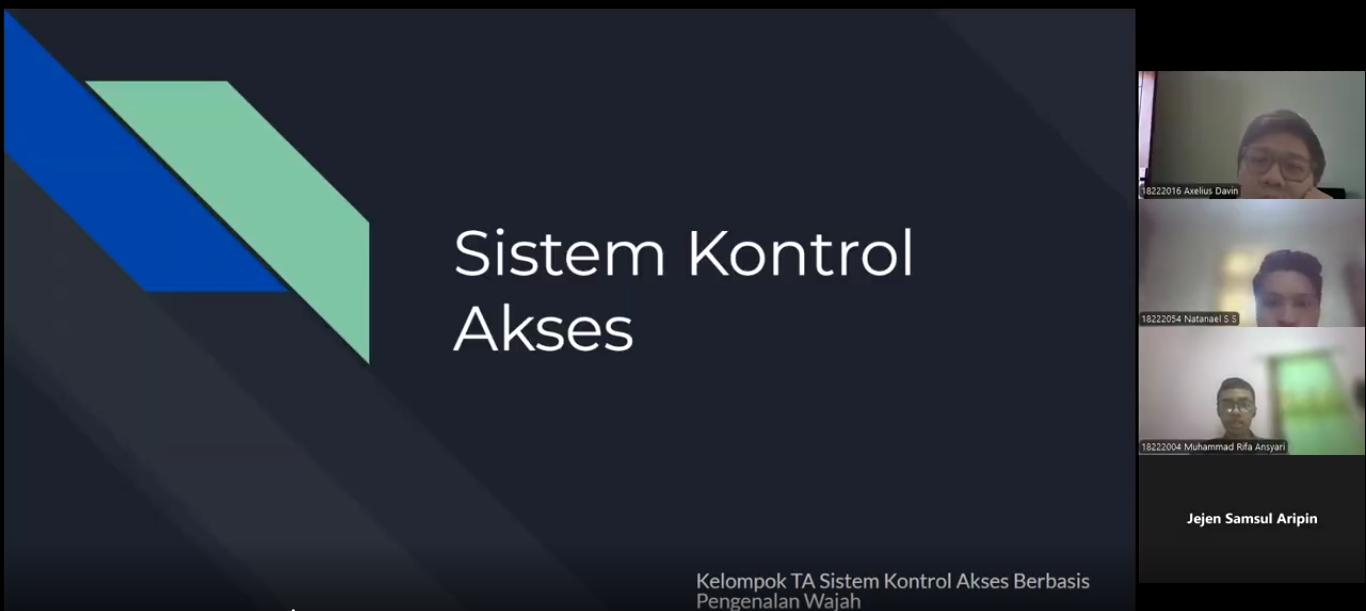
\includegraphics[width=0.6\textwidth]{images/wawancara4_1.png}
    \caption{Dokumentasi Pelaksanaan Wawancara 4 (D)}
\end{figure}

\section{Transkrip Wawancara 4}
Wawancara keempat dilakukan untuk mendalami detail teknis implementasi fitur manajemen tamu dan prosedur akses kredensial perangkat keras. Berikut adalah transkrip lengkap dari diskusi tersebut:

\begin{longtable}{|c|p{0.35\textwidth}|p{0.55\textwidth}|}
\hline
\textbf{No} & \textbf{Pewawancara (Mahasiswa)} & \textbf{Narasumber (Kepala Seksi Data \& SI DKST)} \\ \hline
\endfirsthead
\hline
\textbf{No} & \textbf{Pewawancara (Mahasiswa)} & \textbf{Narasumber (Kepala Seksi Data \& SI DKST)} \\ \hline
\endhead
\hline
\endfoot
\hline
\endlastfoot
1 & Kami berencana membuat \textit{dashboard} manajemen tamu, apakah pendaftaran tamu nanti harus mengisi \textit{form} satu per satu? & Perlu dicari tahu teknisnya. Biasanya di sini cukup perwakilan satu orang saja yang mencatat untuk rombongan (misal: tamu kementerian 10 orang). Tapi di sistem, harus tetap tercatat bahwa jumlah tamu yang masuk adalah 10 orang. Nanti \textit{dashboard} harus bisa menangkap variabel jumlah rombongan tersebut. \\ \hline
2 & Untuk status kehadiran/absensi di \textit{dashboard} karyawan, apakah itu hanya menarik data atau menggantikan sistem absen mesin? & Itu hanya untuk mencatat dan menarik log saja (\textit{check-in/check-out}) dari alat gerbang yang sudah \textit{existing}. Lebih ke memantau statistik karyawan yang hadir hari ini. \\ \hline
3 & Kami berencana mengimplementasikan fitur pendaftaran akun baru melalui web, apakah diperbolehkan? & Kalau memungkinkan, silakan diimplementasikan. Tujuannya memang agar semuanya terpusat. Tapi jika terbatas, untuk tahap pertama buat fitur \textit{view/get data} dulu saja. Tahap keduanya, kalau ada waktu, baru dikembangkan untuk bisa \textit{push data} (nambah/hapus) ke alat gerbang. \\ \hline
4 & Kami mendapat informasi dari Pak Indra bahwa ada server yang terhubung ke gerbang di \textit{basement}, apakah kami bisa mengakses itu juga? & Sebenarnya tidak ada \textit{server} terpusat (tidak ada \textit{cloud} atau \textit{server} khusus). \textit{Server}-nya itu ada di memori lokal (\textit{storage}) masing-masing alat gerbang itu sendiri. Jadi data disimpan di alat yang ada di lobi atau \textit{basement} tersebut. \\ \hline
5 & Oh, jadi di \textit{basement} ada gerbang juga? Bagaimana pelacakan datanya? & Iya, di \textit{basement} ada, tapi sayangnya hanya untuk mendeteksi saat masuk. Saat keluar, alatnya hanya menggunakan tombol \textit{push button} (bukan pemindai wajah/sidik jari), sehingga orang yang keluar dari \textit{basement} tidak akan terdeteksi sistem (\textit{log checkout}-nya hilang). \\ \hline
6 & Jadi untuk mulai mengutak-atik perangkat gerbang ini, apa yang harus kami siapkan? & Silakan buat surat permohonan resmi ke DKST untuk meminta IP dan \textit{User Access} perangkat lobi. Ini formalitas agar seluruh pihak gedung mengetahui. Kalian bisa tanya tim (mahasiswa) kamera untuk \textit{template} suratnya. Kalau sudah dapat izin, PR pertama kalian adalah memastikan apakah kalian bisa mengambil data API langsung dari alat tersebut. \\ \hline
\end{longtable}
